\subsection{Discussion of the Statistical Patterns}
\label{subsec:pattern-discussion}
Logistic regression has the strongest mean validation AUC under both
selectors. CART selection gives it higher sensitivity and F1 (0.761 versus
0.749 for RFE), despite slightly lower AUC. Stacking has lower between-seed
AUC variances (0.000825 with CART and 0.000558 with RFE) than logistic
regression (0.001306 and 0.001930), but also lower discrimination and sensitivity.
Thus, stability alone does not justify the added complexity. The dummy's
perfect sensitivity accompanies zero specificity and accuracy 0.500,
demonstrating why sensitivity cannot be the only criterion.

The implemented ranking uses descending validation AUC, descending accuracy,
and ascending FNR, followed by deterministic name-based tie-breaks. F1,
stability, and interpretability inform the discussion but are not numerical
components of this ranking. Logistic regression wins all five fixed-model
comparisons: CART is selected for seeds 42, 21, and 123, and RFE for seeds
7 and 84. This supports the simpler model family, not a universally best
selector or a claim of statistically significant superiority.

Tuning also selects logistic regression in all five seeds. The selected
$C$ values are 0.1, 0.1, 0.1, 1, and 10 in the stated seed order.
These choices come from training CV and validation, not test performance.
Selection does not guarantee the success criteria: for example, the seed-7
fixed-model winner has validation sensitivity 0.708. Recall is not a hard
eligibility constraint, and threshold optimisation and dedicated calibration
assessment remain unimplemented.

\subsubsection{Interpretation of the Leave-One-Out Results}
\label{subsec:lopo-interpretation}
The LOPO results in Table~\ref{tab:building-lopo-results} show a trade-off
between ranking patients by predicted probability and classifying them at
threshold 0.5. Logistic regression has the highest ROC--AUC (0.874), so it
provides the strongest overall discrimination among the tested models.
Its sensitivity of 0.820 corresponds to identifying 132 of 161 gallstone
records and missing 29; specificity of 0.747 corresponds to correctly
classifying 118 of 158 negative records, with 40 false positives. Thus,
meeting both 0.80 project benchmarks still leaves approximately 18\% of
positive records undetected. AUC alone does not establish calibration or
an acceptable operating threshold.

Random forest performs best at the fixed threshold: accuracy is 0.799,
sensitivity 0.839 and F1 0.808. It detects 135 positive records, misses 26
and produces 38 false positives. Compared with logistic regression, these
aggregate counts represent three fewer missed cases and two fewer false
alarms, despite a lower AUC of 0.857. This makes random forest a useful
candidate for further sensitivity-oriented validation, but the small observed
differences do not establish statistically significant superiority or justify
replacing the validation-selected family after inspecting LOPO results.

Stacking achieves the highest specificity (0.772), with 36 false positives,
but misses 32 positive records: its sensitivity of 0.801 only narrowly meets
the benchmark. Its extra complexity therefore does not deliver the best
case detection. LightGBM offers sensitivity 0.832 with 27 false negatives
and 41 false positives, while XGBoost has the lowest AUC (0.835) and
accuracy (0.762), with 31 false negatives and 45 false positives. All five
predictive models meet the two numerical benchmarks in this pooled run,
but their error trade-offs differ. The dummy's sensitivity of 1.000 is
uninformative without specificity: it incorrectly flags all 158 negative
records. Its unusual pooled AUC is explained below.

\subsubsection{Comparison of Holdout and Leave-One-Out Evaluation}
\label{par:holdout-lopo-discussion}
\begin{table}[H]
\centering\small
\caption{Roles and limitations of the two implemented evaluation methods.}
\label{tab:evaluation-method-comparison}
\begin{tabularx}{\textwidth}{@{}p{2.5cm}XX@{}}
\toprule
Dimension & Repeated stratified holdout & Leave-one-out (LOPO) \\
\midrule
Training and assessment &
223 training, 48 validation and 48 test records per seed. Selected
configurations and test-stage candidate fits use the 271 development records. &
318 training records and one held-out record per fold; 319 folds cover the
whole dataset once for each fixed candidate. \\
Role in this project &
Validation selects the model/selector; training CV selects tuning parameters.
Test results assess fitted candidates or the selected procedure. &
Provides complementary internal assessment of fixed RFE--CART candidates;
it does not repeat the entire model-selection process inside each fold. \\
Coverage and variation &
Five seeds expose split-to-split variation. Validation/test sets contain 48
records each, and records can recur across overlapping splits. &
Each source row contributes one held-out prediction per model. There is one
complete run; heavily overlapping training folds are not independent repeats. \\
Computation &
Fewer outer fits per fixed candidate; tuning and stacking add inner fits. &
319 outer fits per candidate, with additional inner fitting for stacking. \\
Interpretation boundary &
Performance depends on split composition and development size; inspected test
partitions are not a sealed external assessment. &
Uses more training data per prediction, but offers no external validation
and no between-seed variance estimate from the single run. \\
\bottomrule
\end{tabularx}
\end{table}

Table~\ref{tab:holdout-lopo-comparison} compares the same fixed RFE--CART
candidates. Logistic regression's AUC is 0.838 on holdout validation and
0.874 under LOPO, while sensitivity rises from 0.758 to 0.820. Across all
five families, LOPO AUC exceeds mean holdout-validation AUC by approximately
0.036--0.081, and sensitivity by 0.062--0.122. The pattern is consistent
with differences in training size (318 versus 223 records) and assessment
coverage, but this comparison cannot isolate their effects. It is not
evidence that changing the evaluation method improved an otherwise identical
fitted model.

The holdout \emph{test} comparison gives a different picture. Fixed RFE
logistic regression averages AUC 0.887 and sensitivity 0.858 on test,
compared with LOPO's 0.874 and 0.820. LOPO AUC is higher than mean holdout
test AUC for random forest and LightGBM, but lower for logistic regression,
XGBoost and stacking. LOPO sensitivity is lower for all five families.
Consequently, LOPO is not uniformly more favourable. Test fits use 271
development records and assess different, overlapping 48-row subsets;
LOPO evaluates every row with a separate 318-row training set. These
estimates answer related but different questions and should not be ranked
as if they were a controlled model-improvement experiment.

The two methods nevertheless agree that logistic regression has the highest
AUC among fixed RFE candidates. Their threshold-dependent rankings differ:
random forest leads LOPO sensitivity and F1, whereas logistic regression,
XGBoost and stacking share the highest mean RFE holdout-test sensitivity
when rounded to three decimals. This supports keeping discrimination,
sensitivity and false alarms separate in the decision. Use holdout validation
for the stated selection procedure and LOPO as a complementary robustness
check; neither establishes performance on a new cohort. LOPO is
leave-one-person-out only if each source row represents a unique person.
The single run supplies no evidence that LOPO has lower uncertainty than
repeated holdout, and its folds must not be treated as 319 independent
experiments.

\paragraph{Patterns across model families.}
\label{subsec:building-model-patterns}

The tables in Section~\ref{subsec:statistical-patterns} document the outputs for every fixed model. Their
patterns, rather than only the leading score, are summarised in
Table~\ref{tab:building-model-patterns}. Differences between holdout validation
and LOPO reflect different training sizes and evaluation samples; they do not
by themselves establish a statistically significant improvement.

\begin{table}[H]
\centering
\small
\caption{Observed performance patterns for every fixed model and benchmark.}
\label{tab:building-model-patterns}
\begin{tabularx}{\textwidth}{@{}p{2.8cm}X@{}}
\toprule
Model & Pattern and interpretation \\
\midrule
Logistic regression &
Leads validation AUC with either selector and retains the highest LOPO AUC.
CART improves validation sensitivity and F1 relative to RFE. Strong ranking
performance does not eliminate missed cases at threshold 0.5. \\
Random forest &
CART improves validation AUC over RFE without changing mean sensitivity.
Under LOPO it has the highest accuracy, sensitivity, and F1, and lowest FNR
among predictive models, but lower AUC than logistic regression. Its advantage
is threshold-specific case detection rather than the strongest ranking. \\
XGBoost &
CART improves validation AUC and sensitivity over RFE. It has the lowest
LOPO accuracy and AUC among predictive models, so the tested boosting
configuration provides no consistent advantage over simpler alternatives. \\
LightGBM &
CART improves validation AUC while mean sensitivity is unchanged. LOPO
sensitivity exceeds logistic regression's, but AUC and specificity are lower.
It offers a different error balance rather than dominance across metrics. \\
Stacking &
Validation AUC varies less across seeds than logistic regression's but has
a lower mean. LOPO gives the highest specificity and the highest FNR among
predictive models: fewer false alarms accompany more missed positive cases.
Combining models does not automatically improve all outcomes. \\
Training-prior dummy &
Predicts every evaluated row as positive at threshold 0.5. Perfect sensitivity
and zero FNR therefore accompany zero specificity and near-half accuracy;
this is a benchmark failure pattern, not useful disease discrimination. \\
\bottomrule
\end{tabularx}
\end{table}

The tuning experiment also built all four individual model families, not only
the selected logistic models. Their mean validation AUCs were 0.827 for
logistic regression, 0.779 for random forest, 0.777 for XGBoost, and 0.767
for LightGBM, from \protect\path{results/tuning/metrics.csv}. Relative to the fixed
RFE comparison, tuning did not consistently improve external-to-search
validation AUC: logistic regression and LightGBM decreased, random forest
increased slightly, and XGBoost was essentially unchanged at three decimal
places. Training-CV optimisation therefore does not guarantee validation
improvement. Stacking and the dummy were not tuned.

The dummy's pooled LOPO AUC is zero because leaving
out a positive case lowers the training prior while leaving out a negative
raises it, reversing the ranking of the fold-specific probabilities. A fixed
chance score instead has AUC 0.5.

\paragraph{Interpretation of fitted-model associations.}
\label{subsec:model-clinical-patterns}

The following evidence comes from fitted training models and validation perturbations, rather than repeated univariate EDA. Continuous logistic coefficients refer to one training-standard-deviation increase \emph{after} Yeo--Johnson transformation. They describe conditional model associations, not causal effects or original-unit clinical changes. CART rules come from the feature-selection tree, not a surrogate explanation of every ensemble.

\paragraph{Recurring signals and their direction.}
Four predictors recurred in all five 20-feature RFE fits: CRP, vitamin D, the ratio of extracellular fluid to total body water (\texttt{ecf\_tbw}), and haemoglobin. Their mean logistic coefficients were respectively $-1.318$, $+0.690$, $+0.810$ and $+0.549$, with the same sign in every split. CRP ranged from $-1.513$ to $-1.154$ and vitamin D from $+0.569$ to $+0.801$. Thus the fitted models combine laboratory and body-composition information rather than demographic risk alone.

Each raw predictor was also independently shuffled 20 times on each validation partition. Mean AUC decreases across five fits were 0.1127 for CRP, 0.0597 for \texttt{ecf\_tbw}, 0.0437 for vitamin D and 0.0172 for haemoglobin. These quantify perturbation-based contributions, not additive percentages of explained disease risk. The prominence of CRP, vitamin D and bioimpedance measurements agrees with the feature families reported by \textcite{esen2024early}; that study concerns the originating dataset and is not independent replication.

\paragraph{Thresholds and conditional interactions.}
CRP was the root split in all five direct CART selection trees, but its threshold varied: 0.79 for seed 42 and 0.585 for the other four seeds. Table~\ref{tab:clinical-tree-patterns} traces the seed-42 tree before transformation, retaining the recorded dataset scale. Counts describe training nodes, not externally validated risks or calibrated probabilities.



Body-fat ratio separates records within the low-CRP branch, whereas vitamin D separates those within the high-CRP branch. Within the low-CRP, higher-body-fat branch, visceral-fat rating $\leq10.5$ identifies 3/18 positive records, compared with 10/13 above 10.5. This suggests a candidate interaction between overall and visceral adiposity, not an established biological interaction. Different body-composition measures may capture different patient profiles, but these small, adaptively chosen groups require independent confirmation.

Crucially, lower CRP and higher vitamin D correspond to higher predicted gallstone presence here. These directions must not be rewritten as conventional causal risk statements. The outcome is existing gallstones; sampling, treatment or measurement context could affect associations. Learned cut-points are not clinical reference limits. Units and clinical context must be verified before treating any value as a diagnostic threshold; neither increasing CRP nor reducing vitamin D is a supported intervention.

\paragraph{Subgroup differences beyond a global coefficient.}
The female-versus-male logistic contrast was positive in all five models: the mean difference between their one-hot coefficients was $+0.814$, an odds multiplier of approximately 2.26 for that mean contrast, conditional on other transformed predictors. Nevertheless, seed 42's validation model missed 4 of 14 positive female records and 1 of 10 positive male records (27 female and 21 male records overall). A positive demographic coefficient therefore does not ensure equal identification: other covariates can outweigh it. Small denominators support a targeted audit, not a population-level fairness conclusion.

Hepatic-fat grades did not form a monotonic model pattern. Relative to grade 0, mean logistic contrasts were approximately $+0.819$ for grade 1, $-0.535$ for grade 2 and $-0.460$ for grade 3. These models therefore do not establish that increasing hepatic-fat severity increases gallstone risk. Conditional associations, sparse categories and overlapping metabolic measurements are competing explanations requiring clinical review.

\paragraph{Why weaker predictors contribute less.}
Selection alone does not establish useful prediction. Alkaline phosphatase was retained in all five RFE fits, yet its mean coefficient was only $-0.081$, changed sign across fits, and its mean validation permutation contribution was $-0.0024$. Triglycerides appeared in three fits, had mean coefficient $+0.013$ when selected, and mean perturbation contribution $-0.0055$ across all five fits. Negative contributions mean shuffling slightly improved validation discrimination, consistent with unstable or unnecessary fitted information; they do not indicate a protective clinical effect.

An excluded variable necessarily has zero permutation contribution in that pipeline. Age was excluded in every reference fit: this demonstrates non-use by the selector, not clinical irrelevance. Correlated measurements may substitute for each other, and single-variable permutation can understate shared information. RFE also ranks usefulness to CART, which need not match usefulness to the downstream logistic model.

The strongest signal is concentrated in CRP, but complementary contributions remain in fluid balance, vitamin D and smaller laboratory or categorical effects. The later 10-feature comparison in Section~\ref{subsec:iterations} tests retention of information in aggregate; it does not prove that every retained variable is necessary or identify which removed variable caused the loss. Grouped ablation would be needed to distinguish shared body-composition information from unique contributions.

\subsection{Visualisation of Model Patterns}
\label{subsec:pattern-visualisation}
\begin{figure}[H]
\centering
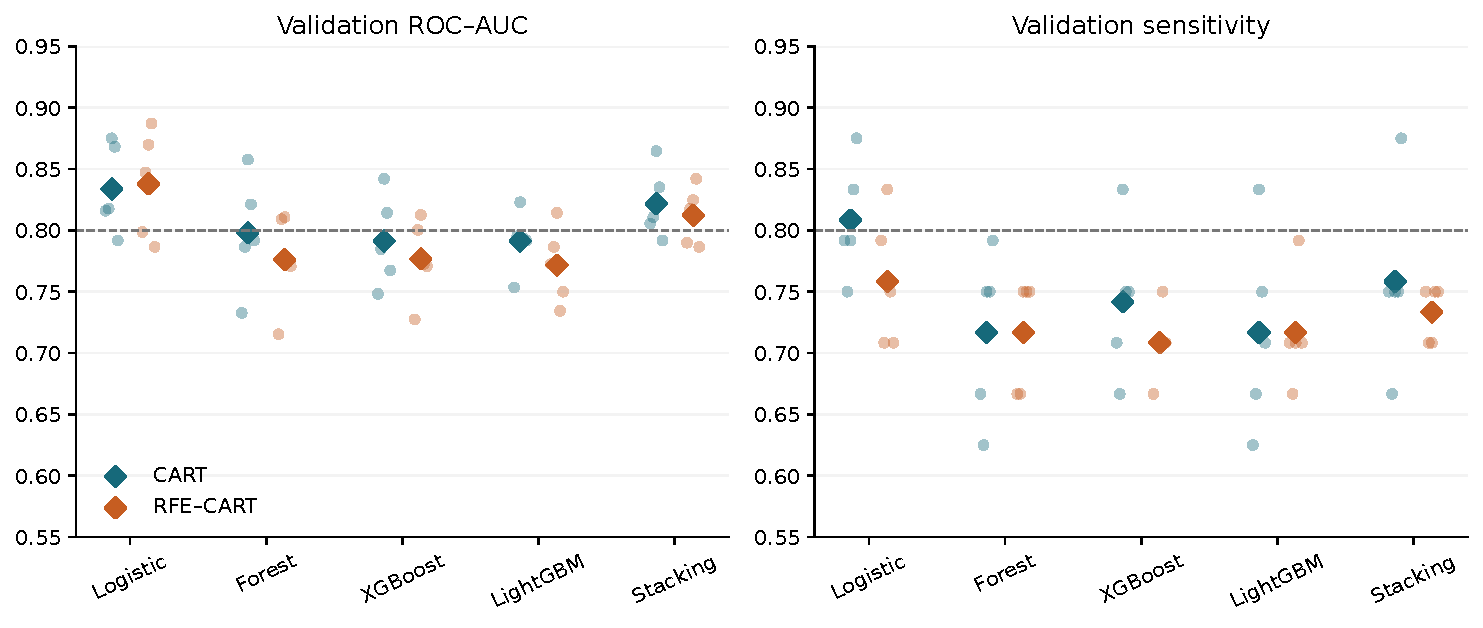
\includegraphics[width=\textwidth]{figures/modeling/model_comparison.pdf}
\caption{Validation discrimination and sensitivity for every predictive family
and selector. Large markers show five-seed means; small markers show individual
seeds, not confidence intervals. Dashed lines indicate the project benchmarks.
Source: \protect\path{results/holdout/metrics.csv}.}
\label{fig:model-comparison}
\end{figure}
\begin{figure}[H]
\centering
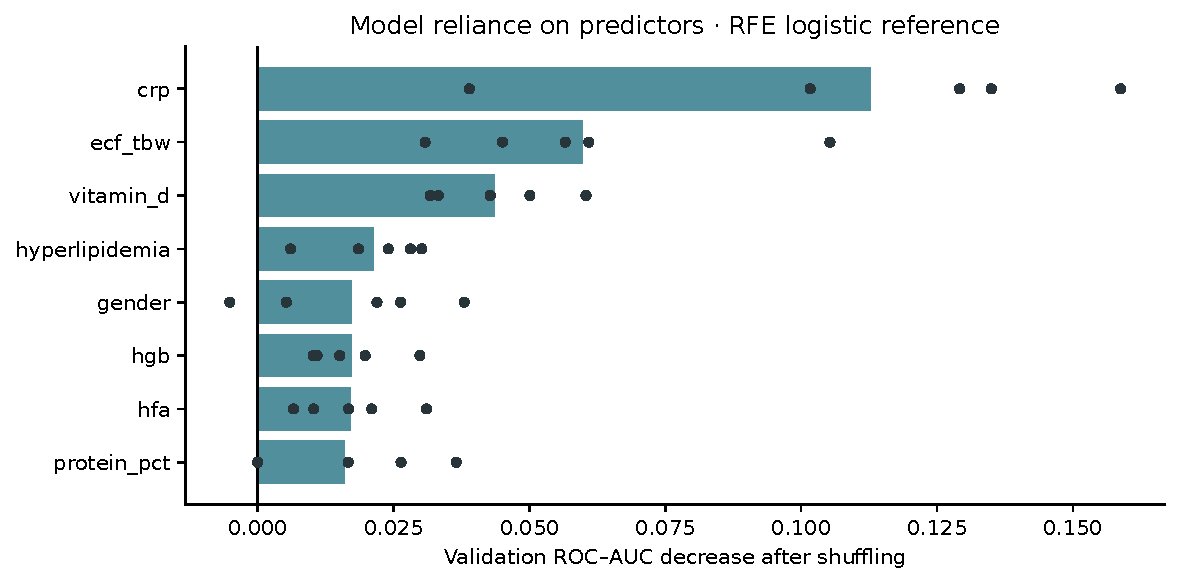
\includegraphics[width=0.93\textwidth]{figures/modeling/permutation_patterns.pdf}
\caption{Largest mean validation permutation contributions in the 20-feature
RFE logistic reference. Bars are mean AUC decreases; points are five fitted
splits, each averaging 20 shuffles. Correlated fields can share information;
these values are neither causal effects nor additive risk percentages.
Source: \protect\path{results/iteration_patterns/permutation.csv}.}
\label{fig:permutation-patterns}
\end{figure}
\subsection{Error Analysis: Repeatedly Misclassified Records}
\label{subsec:building-repeated-errors}

The saved prediction files permit review of errors that recur across seeds
and model families. Table~\ref{tab:building-repeated-errors} uses the
\emph{validation-selected fixed model} for each holdout seed, identified by
\protect\path{results/holdout/validation_winners.csv}, and its test predictions in
\protect\path{results/holdout/predictions.csv}. All these selected models are logistic
regression. Probabilities refer to gallstones being present; predictions use
threshold 0.5. The examples were chosen retrospectively to illustrate errors,
not to estimate their prevalence in future patients.

\begin{table}[H]
\centering
\small
\caption{Examples of repeated held-out errors; denominators count eligible test appearances.}
\label{tab:building-repeated-errors}
\begin{tabular}{@{}rlcrrr@{}}
\toprule
Source row & Holdout seeds & Error & Errors/runs & Probability range & LOPO errors/models \\
\midrule
117 & 7, 42      & FN & 2/2 & 0.068--0.350 & 4/5 \\
291 & 21, 42, 84 & FP & 3/3 & 0.703--0.758 & 5/5 \\
316 & 7, 84, 123 & FP & 3/3 & 0.634--0.794 & 5/5 \\
\bottomrule
\end{tabular}
\end{table}

\textbf{Record 117} has gallstones but was predicted absent in both holdout
test appearances. In LOPO, logistic regression, random forest, XGBoost, and
stacking also missed it; LightGBM correctly classified it with probability
0.566. The tuned holdout winners still missed it in both seeds. This is a
recurring false-negative example, although the LightGBM result shows that
the error is not universal across models.

\textbf{Records 291 and 316} have no gallstones but were repeatedly predicted
positive. Across all five predictive families and both selectors, record 291
was wrong in 29/30 holdout predictions and record 316 in 30/30; both were
false positives for all five LOPO models. Tuning corrected record 291 only
in seed 42, with probability 0.491, just below the decision threshold,
whereas record 316 remained wrong in all three tuned test appearances.
The first correction is therefore a borderline classification change, not
evidence that tuning consistently resolves the record's errors.

These identifiers are zero-based \texttt{source\_row} values, not verified
patient IDs. Repetition means the same dataset record was tested in several
overlapping splits or by different models, not that a patient had repeated
clinical visits. The LOPO denominator excludes the dummy benchmark. Shared
errors across model families motivate review of source measurements, labels,
and overlapping predictor profiles, but do not prove mislabelling or a causal
explanation. Their review must not be used to retune models and then claim
independent performance on the same test records.

\subsection{Model Evaluation Against the Project Objectives}
\label{subsec:model-evaluation}
\begin{table}[H]
\centering\small
\caption{Internal test performance of the validation-selected fixed procedure across five seeds. Ranges describe split variation, not confidence intervals.}
\begin{tabular}{lll}
\toprule
Metric & Mean & Minimum--maximum \\
\midrule
ROC--AUC & 0.883 & 0.828--0.915 \\
Sensitivity & 0.892 & 0.792--0.958 \\
Specificity & 0.708 & 0.667--0.792 \\
F1 & 0.816 & 0.769--0.846 \\
\bottomrule
\end{tabular}
\end{table}

These results come from \path{results/holdout/selected_test_metrics.csv}; selectors vary by seed. They describe the selected procedure, whereas the all-candidate tables in Section~\ref{subsec:statistical-patterns} describe individual models. Reused, overlapping test partitions limit independence.

The selected family is logistic regression, chosen using validation rather
than test ranking. Mean scores can meet a benchmark while individual splits
fail it. At the fixed 0.5 threshold, the RFE logistic reference has mean
validation AUC 0.838 but sensitivity 0.758: discrimination meets 0.80,
whereas case detection does not. The CART logistic candidate has means
0.834 and 0.808, but this does not establish reliable performance for every
split. LOPO logistic AUC 0.874 and sensitivity 0.820 are complementary
internal results for a fixed candidate, not a nested evaluation of selection.
The 20-feature RFE reference is consequently used for a controlled follow-up
experiment in Section~\ref{subsec:iterations}; it is not claimed to be the
selected selector in every seed.

\paragraph{Final fitting and evaluation integrity.}
\label{subsec:model-selection-feedback}

Selected configurations are refitted on the 271 development rows before
assessment on the 48 test rows. Complete pickle pipelines preserve preparation
and classifier state in \protect\path{models/holdout/} and \protect\path{models/tuned/}.
LOOCV evaluates fixed candidate pipelines by holding out each row once;
\protect\path{models/lopo/} contains separate full-data refits for future inference.
It is row-level evaluation, and it is not nested evaluation of the entire
algorithm-selection procedure.

The Iteration 2 concern is \textbf{partly resolved}: automatic selection now
excludes test scores, and the model-building argument above uses validation
evidence. However, the fixed-model notebook still evaluates every candidate
on test before recording its validation winner, and tuning reuses those
partitions. The resulting exposure permits informal test-driven decisions.
Overlapping splits and prior dataset exploration further limit independence;
the results must be described as internal evaluations.

A stricter future workflow would lock the complete configuration before
accessing an untouched test set and evaluate only that configuration.
Alternatively, nested outer evaluation should contain all selection decisions
within its training folds. Error analysis may motivate later revisions, but
revised models require new assessment. This qualification addresses the
feedback without claiming that the current implementation provides a fully
sealed final test.

\paragraph{Decision and feedback trigger.}
Retain logistic regression as the leading research family, but do not claim
that the current workflow establishes deployment readiness. Calibration,
threshold selection, generalisation and the cost of false positives remain
unresolved. Variable sensitivity and recurring errors motivate returning to
feature selection after this evaluation. The next subsection records the
completed controlled revision, including its unsuccessful outcome.
\subsection{A Completed CRISP-DM Feedback Cycle}
\label{subsec:iterations}

The Python/Jupyter workflow follows CRISP-DM as a feedback cycle. The business objective remains to support assessment of gallstone presence, with missed cases a particular concern; this is not a prospective disease-onset model. Sections~\ref{sec:model-building} and~\ref{subsec:model-evaluation} report execution evidence and the model evaluation. Here, evaluation motivates a return to feature selection, followed by an executed rerun and a documented decision.

\paragraph{Cycle A: establish and evaluate the reference.}
Data understanding established the coded categories and outcome direction: source status 0 becomes modelling class 1 (gallstones present). Data preparation fitted imputation, CART-based recursive feature elimination (RFE; 20 predictors), Yeo--Johnson transformation and standardisation on each training partition. Logistic regression used $C=1$ and a 0.5 classification threshold. Five stratified 70--15--15 splits used seeds 42, 7, 21, 84 and 123, with 223 training, 48 validation and 48 test records each. Evaluation exposed variable sensitivity and recurring errors, prompting the question: does a smaller predictor set remove unstable information without losing useful signal?

\paragraph{Cycle B: revisit preparation, rebuild and re-evaluate.}
A focused revision reduced RFE from 20 to 10 predictors. This was the only changed modelling choice: rows, seeds, transformations, logistic settings and threshold remained fixed. All preprocessing and feature selection were fitted again on the 223 training records, and both cycles were rerun on the corresponding validation records. No test records were evaluated in this additional experiment. This completes the loop
\emph{evaluation $\rightarrow$ revised data preparation $\rightarrow$ modelling $\rightarrow$ evaluation $\rightarrow$ decision}, rather than merely proposing future work.

\begin{table}[htbp]
\centering
\small
\caption{Paired validation comparison. Summary entries are mean $\pm$ sample variance across five seeds, not standard deviation. Bold indicates the higher mean or seed-level value.}
\label{tab:iteration-summary}
\begin{tabular}{lrrrr}
\toprule
& \multicolumn{2}{c}{Validation AUC} & \multicolumn{2}{c}{Sensitivity} \\
Seed & 20 features & 10 features & 20 features & 10 features \\
\midrule
42  & \textbf{0.799} & 0.760 & \textbf{0.792} & \textbf{0.792} \\
7   & \textbf{0.847} & 0.825 & \textbf{0.708} & 0.667 \\
21  & \textbf{0.870} & 0.826 & \textbf{0.833} & 0.750 \\
84  & \textbf{0.887} & 0.856 & \textbf{0.750} & \textbf{0.750} \\
123 & 0.786 & \textbf{0.811} & 0.708 & \textbf{0.792} \\
\midrule
Mean $\pm$ variance &
$\mathbf{0.838}\pm0.001930$ & $0.816\pm0.001223$ &
$\mathbf{0.758}\pm0.002951$ & $0.750\pm0.002604$ \\
\bottomrule
\end{tabular}
\end{table}


\begin{figure}[H]
\centering
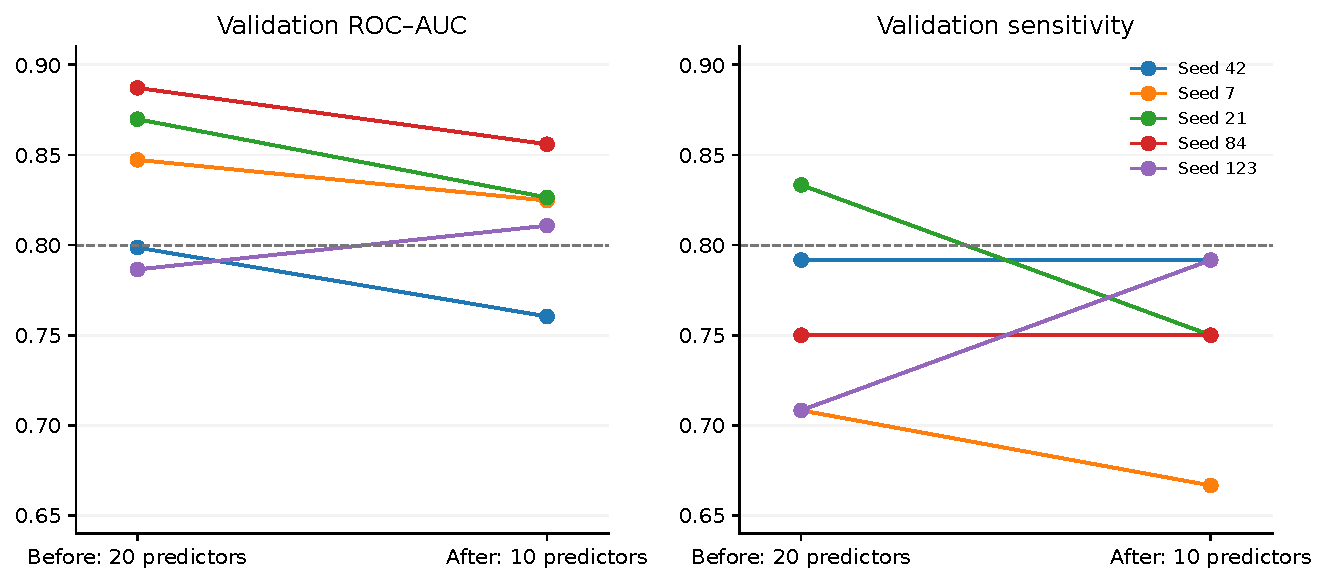
\includegraphics[width=\textwidth]{figures/modeling/iteration_comparison.pdf}
\caption{Completed feedback cycle: paired validation results before and after
reducing RFE from 20 to 10 predictors. Each line connects the same seed;
all other modelling choices are held fixed. Dashed lines mark the 0.80
project targets. Source: \protect\path{results/iteration_patterns/cycle_metrics.csv}.}
\label{fig:iteration-comparison}
\end{figure}

\paragraph{Decision and robustness boundary.}
The revision lowered AUC in four of five splits, with a mean change of $-0.0222$; sensitivity fell by 0.0083 on average. Lower between-seed variance did not compensate for lower discrimination or resolve missed cases. The 20-feature reference was therefore retained for this comparison. This tests robustness to a specific simplification, not universal superiority: validation partitions overlap across seeds, have already informed development, and neither cycle achieved mean sensitivity of 0.80. The revised model was not promoted to the saved candidate folders. Separate tuning and LOPO results remain in Sections~\ref{subsec:parameter-settings} and~\ref{subsec:statistical-patterns}; they are not independent external confirmation of this iteration.

\paragraph{Proposed next feedback cycle.}
The completed comparison shows that reducing the number of predictors alone
does not resolve missed cases. Table~\ref{tab:next-dm-cycle} translates this
finding and the remaining evaluation gaps into specific preparation and
modelling changes. These are proposed experiments, not additional completed
cycles. Each experiment should record its motivating finding, controlled
change, evaluation result and retain-or-reject decision.

\begin{table}[htbp]
\centering
\small
\caption{Proposed changes for the next CRISP-DM feedback cycle.}
\label{tab:next-dm-cycle}
\begin{tabularx}{\textwidth}{@{}p{2.3cm}XX@{}}
\toprule
Area & Proposed change and rationale & Evaluation and decision rule \\
\midrule
Feature engineering &
Test a small, prespecified set of representations or interactions, such as
overall-by-visceral adiposity, motivated by conditional model patterns.
Verify units and measurement availability; distinguish existing ratios from
newly engineered features. &
Compare against the unchanged logistic reference using paired development
folds. Fit transformations within training folds and retain changes only
when validation supports their contribution. \\
\addlinespace
Feature importance &
Use grouped permutation and refitted group ablation for correlated fluid,
adiposity and laboratory measurements, extending individual importance
estimates. &
Compare AUC, sensitivity and stability. Distinguish a fitted model's reliance
on a variable group from the performance achievable after refitting without
it; low individual importance alone does not justify removal. \\
\addlinespace
Feature selection &
Compare the 20-feature RFE reference with logistic-compatible selection,
regularised logistic regression using all eligible predictors, and a
predefined routine-measurement subset. &
Choose feature counts and penalties within inner development folds. Assess
performance and measurement burden together; the unsuccessful 10-feature
revision does not establish that every retained field is necessary. \\
\addlinespace
Calibration and threshold &
Assess probability calibration and select a threshold using a prespecified
sensitivity target and an agreed specificity or assessment-workload
constraint. &
Fit any calibrator and choose the threshold within development data using
held-out predictions. Freeze both before outer evaluation; report
calibration, sensitivity, specificity and confusion counts. \\
\addlinespace
Subgroup evaluation &
Extend the preliminary sex-specific error review to predefined sex and age
groups, checking measurement quality and sample support. &
Report group sizes, positive counts, error rates and uncertainty. Small
groups support further investigation rather than firm fairness claims. \\
\bottomrule
\end{tabularx}
\end{table}

All feature, model, calibration and threshold choices must remain inside the
development process. Because the current test partitions have already been
inspected, subsequent results on those records remain exploratory. Nested
evaluation can assess a prespecified selection procedure internally, while an
untouched external cohort is needed to examine transfer beyond this dataset.
If no candidate satisfies the predefined success criteria, the next cycle
should report that outcome rather than select a model by AUC alone.

\subsection{Return to Business Understanding and Deployment}
\label{subsec:business-objective-evaluation}

The completed cycle supports a research screening aid, not deployment or replacement of clinical assessment. Simplification can sacrifice complementary information without resolving false negatives. Repeatedly misclassified records documented in Section~\ref{subsec:building-repeated-errors} should guide source-data and subgroup review, not retrospective relabelling. The next CRISP-DM cycle should specify calibration and sensitivity-oriented threshold selection within development data, then assess the frozen pipeline on an untouched external cohort. These steps are planned, not claimed as completed.

\paragraph{Reproducibility.}
The executed comparison and pattern extraction are implemented in
\protect\path{scripts/iteration_pattern_analysis.py}, using the existing \protect\path{utils.py}.
The folder \protect\path{results/iteration_patterns/} records per-seed cycle results,
sample variances, selected fields, coefficients, validation permutation
contributions, subgroup counts, CART node counts and the source-data signature.
The analysis refits training-specific transformations from raw records; it does
not evaluate the full-data reference transformed CSV.
